\documentclass[11pt]{article}
\usepackage[utf8]{inputenc}
\usepackage[T1]{fontenc}
\usepackage{amsmath}
\usepackage{amsfonts}
\usepackage{geometry}
\usepackage{hyperref}
\usepackage{titlesec}
\usepackage{graphicx}
\usepackage{float}
\usepackage{booktabs}
\usepackage{multicol}
\usepackage{enumitem}

\geometry{a4paper, margin=0.85in}

\titleformat{\section}{\large\bfseries}{}{0em}{}[\titlerule]
\titleformat{\subsection}{\bfseries}{}{0em}{}
\setlength{\parskip}{3pt}
\setlength{\parindent}{0pt}

\begin{document}

% --- TITLE PAGE ---
\begin{titlepage}
	\centering
	\vspace*{2cm}
	\Huge\textbf{IKT215 Assignment 3: \\ Function Approximation Classification, \\ Error Estimation and Model Selection} \\
	\vspace{1.5cm}
	\Large \textbf{Student:} Gomery K. Wanjiru \\
	\Large \textbf{Course:} IKT215 \\
	\vfill
	\section*{Disclaimer on Generative AI}
	In accordance with UiA's guidelines, I declare that I used Generative AI tools to assist in structuring the LaTeX report and generating boilerplate code for plotting and data loading. The neural network implementation, error estimation analysis, model selection methodology, and interpretation of results are my own work, guided by the course lecture materials (Lectures 6--8) and exercises (7--9).
\end{titlepage}

\newpage
\section{Introduction}
This report presents a neural network-based classification system for the mfeat-factors dataset, which contains 216 profile correlation features extracted from handwritten digits (0--9) from Dutch utility maps. The assignment covers four parts: data exploration and preparation, neural network implementation, comparison of error estimation techniques, and model selection strategies.

All experiments use PyTorch for neural network implementation and scikit-learn for data preprocessing and evaluation utilities. The dataset is pre-split into 1600 training and 400 test samples, with perfectly balanced classes (160/40 samples per class for train/test respectively).

\section{Part 1: Setup and Exploration}

The mfeat-factors dataset was loaded from the provided \texttt{.npz} files. Table~\ref{tab:data_summary} summarizes the dataset characteristics.

\begin{table}[H]
	\centering
	\caption{Dataset summary.}
	\begin{tabular}{lcc}
		\toprule
		Property          & Training Set & Test Set  \\
		\midrule
		Samples           & 1600         & 400       \\
		Features          & 216          & 216       \\
		Classes           & 10 (0--9)    & 10 (0--9) \\
		Samples per class & 160          & 40        \\
		Feature range     & [0, 1353]    & ---       \\
		\bottomrule
	\end{tabular}
	\label{tab:data_summary}
\end{table}

\textbf{Normalization.} Since the raw features span a wide range ($[0, 1353]$, mean $\approx 318$, std $\approx 352$), I applied \textbf{standardization} (zero mean, unit variance) using \texttt{StandardScaler}. The scaler was fitted on the training data only to prevent information leakage. After normalization, the training set has mean $\approx 0.0$ and std $\approx 1.0$, while the test set has mean $\approx -0.005$ and std $\approx 1.007$, confirming proper scaling. The classes are perfectly balanced, so no resampling was needed.

\section{Part 2: Neural Network Implementation}

\subsection{Architecture}
I implemented a fully connected neural network in PyTorch with the following architecture:

\begin{table}[H]
	\centering
	\caption{Network architecture (primary model, Config B).}
	\begin{tabular}{lccl}
		\toprule
		Layer           & Input & Output & Details                       \\
		\midrule
		Linear + BN     & 216   & 128    & BatchNorm, ReLU, Dropout(0.3) \\
		Linear + BN     & 128   & 64     & BatchNorm, ReLU, Dropout(0.3) \\
		Linear (output) & 64    & 10     & Raw logits (softmax in loss)  \\
		\bottomrule
	\end{tabular}
	\label{tab:architecture}
\end{table}

Total trainable parameters: \textbf{37,066}. The design choices are motivated by the lectures:
\begin{itemize}[nosep]
	\item \textbf{ReLU activation}: Non-saturating nonlinearity that avoids the vanishing gradient problem (Lecture 6, slide 50).
	\item \textbf{Batch normalization}: Stabilizes training by normalizing layer inputs, enabling higher learning rates.
	\item \textbf{Dropout (0.3)}: Regularization to reduce overfitting, acting as an implicit ensemble.
	\item \textbf{Cross-entropy loss}: Appropriate for multi-class classification using softmax outputs (Lecture 6, slide 41--42).
\end{itemize}

\subsection{Training Approach}
\begin{itemize}[nosep]
	\item \textbf{Optimizer}: Adam with learning rate $\eta = 0.001$ and weight decay $10^{-4}$.
	\item \textbf{Batch size}: 64 (mini-batch SGD for faster convergence, Lecture 6, slide 52).
	\item \textbf{Learning rate schedule}: ReduceLROnPlateau (halves LR after 10 epochs without improvement).
	\item \textbf{Early stopping}: Training stops after 25 epochs without validation loss improvement, and the best model (by validation loss) is restored.
	\item \textbf{Validation split}: 80/20 stratified split of training data.
\end{itemize}

The model converged within $\sim$105 epochs. Training and validation curves (Figure~\ref{fig:training_curves}) show smooth convergence with no significant overfitting gap.

\begin{figure}[H]
	\centering
	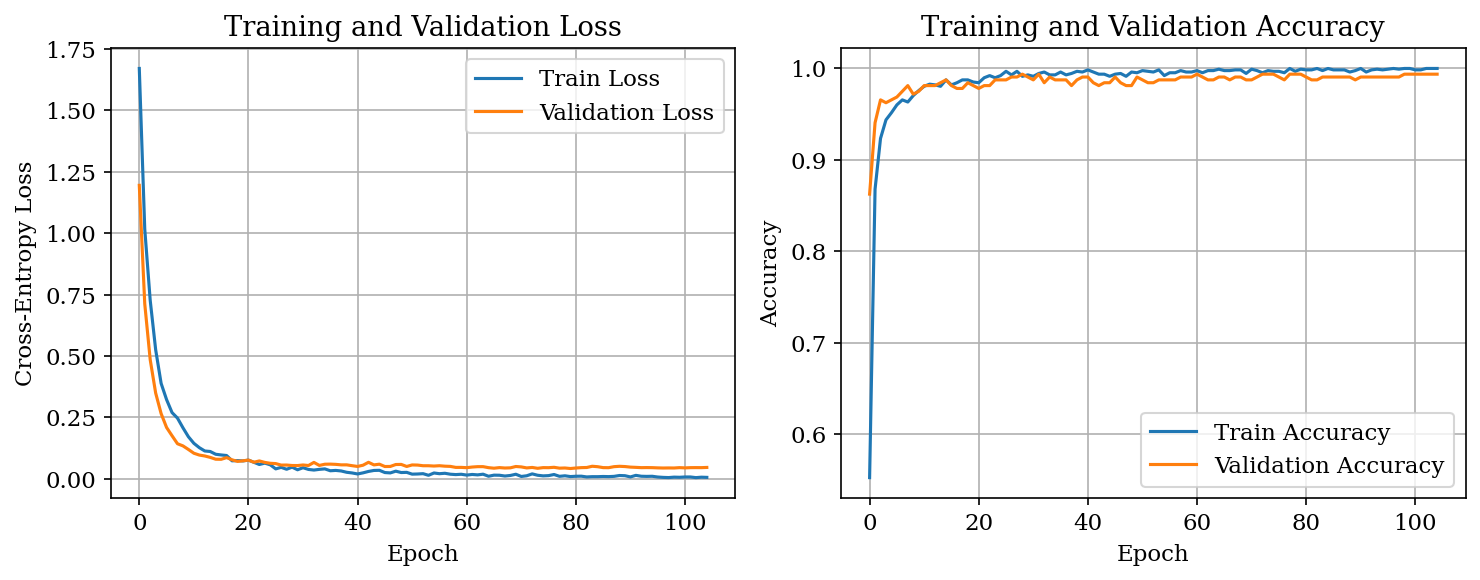
\includegraphics[width=0.85\textwidth]{training_curves.png}
	\caption{Training and validation loss/accuracy curves. The model converges around epoch 50 with early stopping triggered at epoch 105.}
	\label{fig:training_curves}
\end{figure}

\textbf{Test performance:} The model achieves \textbf{97.75\%} accuracy on the held-out test set (error rate: 2.25\%). Figure~\ref{fig:confusion_matrix} shows the confusion matrix. The most common errors involve digits 1 and 5 (3 misclassifications each), which are visually similar in handwritten form.

\begin{figure}[H]
	\centering
	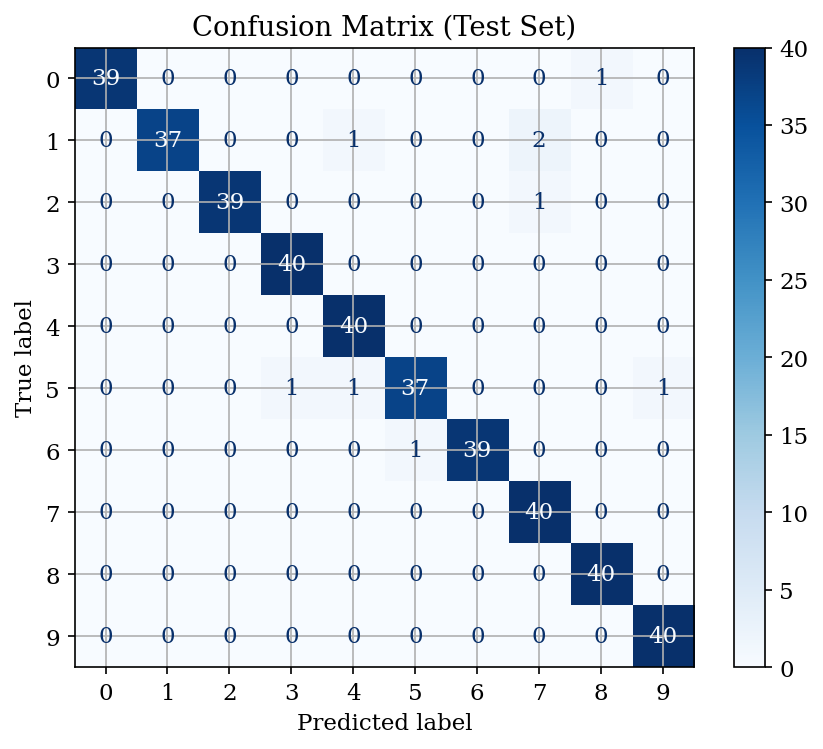
\includegraphics[width=0.42\textwidth]{confusion_matrix.png}
	\caption{Confusion matrix on the test set. Most classes achieve near-perfect classification.}
	\label{fig:confusion_matrix}
\end{figure}

\section{Part 3: Error Estimation}

I implemented three error estimation techniques using the same network architecture (Config B: 128-64, dropout 0.3) and compared them against the true test error.

\subsection{Resubstitution Error}
The classifier is trained on \emph{all} $n = 1600$ training samples and evaluated on the \emph{same} training data (Lecture 7, slide 7):
$$\hat{\varepsilon}_n^{\text{resub}} = \frac{1}{n} \sum_{i=1}^{n} |Y_i - \psi_n(\mathbf{X}_i)|$$

\textbf{Result:} Resubstitution error = \textbf{0.00\%} (accuracy 100\%).

The model achieves perfect training accuracy, a dramatically optimistic estimate compared to the true test error of 1.75\%. As discussed in Lecture 7 (slide 23), the resubstitution estimator has $\text{Bias}(\hat{\varepsilon}_n) < 0$ (optimistically biased) because the classifier is evaluated on the same data used for design. A neural network with 37,066 parameters and only 1,600 samples has ample capacity to memorize the training set, producing $\hat{\varepsilon}_n^{\text{resub}} = 0$ even when the true error is substantially higher.

\textbf{Advantage:} Fastest estimation; no additional data needed. \textbf{Limitation:} Severely underestimates the true error, especially for high-capacity models; unacceptably large bias in small-sample situations (Lecture 7, slide 23).

\subsection{Hold-Out Error}
The training data is split 80/20 into a design set ($n{-}m = 1280$ samples) and a hold-out set ($m = 320$ samples). The classifier is trained on the design set and evaluated on the hold-out set (Lecture 7, slide 18--21).

\textbf{Result:} Hold-out error = \textbf{0.62\%} (accuracy 99.38\%).

While the hold-out estimator is unbiased given the training data, $E[\hat{\varepsilon}_{n,m} \mid S_n] = \varepsilon_n$ (Lecture 7, slide 19), its RMS is distribution-independently bounded by (Lecture 7, slide 20):
$$\text{RMS}(\hat{\varepsilon}_{n,m}) \leq \frac{1}{2\sqrt{m}} = \frac{1}{2\sqrt{320}} \approx 2.80\%$$
This means the hold-out estimate could deviate from the true error by up to 2.80\% in the worst case. The observed deviation is $|0.62\% - 1.75\%| = 1.13\%$, within this bound.

The hold-out error (0.62\%) substantially underestimates the true test error (1.75\%). This gap arises because the hold-out set is drawn from the \emph{same} original collection as the training data. During data collection, all 2000 samples were gathered together, and the train/hold-out split is random within this set. In contrast, the external test set may exhibit slightly different characteristics. Additionally, training on 1280 samples (instead of the full 1600) reduces classifier quality, yet the hold-out set shares the same sampling conditions, making the classifier appear better on this particular split.

\textbf{Advantage:} Unbiased conditional on training data; bounded RMS. \textbf{Limitation:} Reduces training data; high variance from a single split; estimate depends on the particular partition chosen.

\subsection{5-Fold Cross-Validation}
The training data is partitioned into 5 equal folds. For each fold, the model is trained on 4 folds (1280 samples) and evaluated on the remaining fold (320 samples). The average error across folds gives the CV estimate (Lecture 7, slide 9).

\textbf{Result:} CV error = \textbf{2.50\% $\pm$ 0.44\%}.

Table~\ref{tab:cv_folds} shows the per-fold breakdown, demonstrating moderate stability across partitions.

\begin{table}[H]
	\centering
	\caption{Per-fold 5-fold cross-validation results.}
	\begin{tabular}{lccc}
		\toprule
		Fold                    & Train Size & Test Size & Error Rate                   \\
		\midrule
		1                       & 1280       & 320       & 2.19\%                       \\
		2                       & 1280       & 320       & 2.81\%                       \\
		3                       & 1280       & 320       & 1.88\%                       \\
		4                       & 1280       & 320       & 3.12\%                       \\
		5                       & 1280       & 320       & 2.50\%                       \\
		\midrule
		\textbf{Mean $\pm$ Std} &            &           & \textbf{2.50\% $\pm$ 0.44\%} \\
		\bottomrule
	\end{tabular}
	\label{tab:cv_folds}
\end{table}

This is the closest estimate to the true test error (1.75\%). As expected from theory (Lecture 7, slides 24--25), $k$-fold CV has near-unbiasedness: $E[\hat{\varepsilon}_n] = E[\varepsilon_{n - n/k}]$. Since each fold trains on only 80\% of the data ($n - n/k = 1280$), the CV estimate is \emph{pessimistically} biased: $E[\varepsilon_{1280}] > E[\varepsilon_{1600}]$, because a classifier trained on fewer samples generally has higher error. This explains why the CV error (2.50\%) slightly exceeds the true test error (1.75\%). The fold-to-fold standard deviation of 0.44\% reflects the variance inherent in both the random partitioning and the instability of neural network training.

\textbf{Advantage:} Uses all data for both training and evaluation; near-unbiased; provides variance estimate. \textbf{Limitation:} Computationally expensive ($k\times$ training); pessimistically biased due to smaller training sets; variance can be large for unstable classifiers (Lecture 7, slide 26).

\begin{figure}[H]
	\centering
	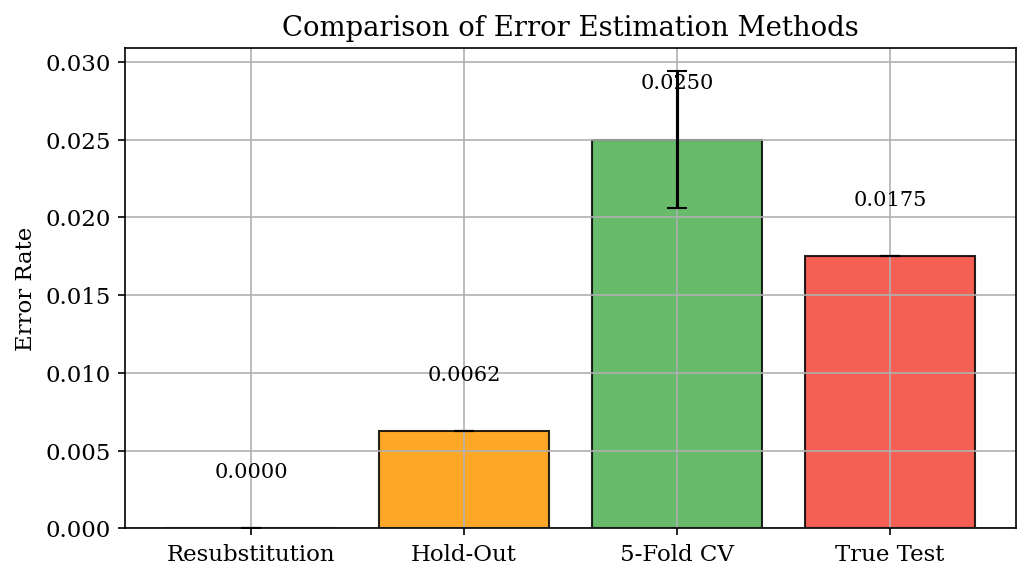
\includegraphics[width=0.65\textwidth]{error_estimation_comparison.png}
	\caption{Comparison of error estimation methods. Resubstitution achieves 0\% error (severe optimistic bias), hold-out underestimates at 0.62\%, and 5-fold CV (2.50\%) closely brackets the true test error (1.75\%) with slight pessimistic bias.}
	\label{fig:error_comparison}
\end{figure}

\subsection{Summary}
\begin{table}[H]
	\centering
	\caption{Error estimation results.}
	\begin{tabular}{lcc}
		\toprule
		Method           & Error Rate          & Bias Direction       \\
		\midrule
		Resubstitution   & 0.00\%              & Optimistic           \\
		Hold-Out (80/20) & 0.62\%              & Optimistic           \\
		5-Fold CV        & 2.50\% $\pm$ 0.44\% & Slightly pessimistic \\
		True Test Error  & 1.75\%              & ---                  \\
		\bottomrule
	\end{tabular}
	\label{tab:error_est}
\end{table}

The results confirm the theoretical hierarchy: resubstitution is severely optimistically biased ($\text{Bias} < 0$, Lecture 7, slide 23), hold-out improves on this but remains optimistic due to single-split variance, and cross-validation provides the most reliable estimate by averaging over multiple splits. The RMS bound for hold-out with $m = 320$ is $\leq 2.80\%$ (Lecture 7, slide 20), and the CV pessimistic bias $E[\varepsilon_{1280}] > E[\varepsilon_{1600}]$ explains why CV slightly overshoots the true error.

\section{Part 4: Model Selection}

I compared three network configurations (Table~\ref{tab:configs}) using two model selection approaches.

\begin{table}[H]
	\centering
	\caption{Network configurations compared for model selection.}
	\begin{tabular}{lccccc}
		\toprule
		Configuration     & Hidden 1 & Hidden 2 & Dropout & LR     & Parameters \\
		\midrule
		Config A (Small)  & 64       & 32       & 0.2     & 0.001  & 16,490     \\
		Config B (Medium) & 128      & 64       & 0.3     & 0.001  & 37,066     \\
		Config C (Large)  & 256      & 128      & 0.4     & 0.0005 & 90,506     \\
		\bottomrule
	\end{tabular}
	\label{tab:configs}
\end{table}

\subsection{Train-Validation-Test Approach}
The training data was split into three sets: training (70\%, 1120 samples), validation (15\%, 240 samples), and an internal test set (15\%, 240 samples). Each configuration was trained on the training portion, the best model was selected by validation accuracy, and the final performance was assessed on the external test set (Lecture 8, slide 16).

\begin{table}[H]
	\centering
	\caption{Train-Validation-Test results.}
	\begin{tabular}{lccc}
		\toprule
		Configuration     & Val Acc         & Internal Test Acc & Final Test Acc  \\
		\midrule
		Config A (Small)  & 0.9917          & 0.9833            & \textbf{0.9800} \\
		Config B (Medium) & \textbf{1.0000} & 0.9792            & 0.9750          \\
		Config C (Large)  & 0.9917          & 0.9833            & 0.9700          \\
		\bottomrule
	\end{tabular}
\end{table}

Config B was selected with the highest validation accuracy (100\%). The final test accuracy is 97.50\%. However, by the selection probability theorem (Lecture 8, slide 14), the probability of making a wrong selection satisfies:
$$P\big(\varepsilon(\psi_n) - \varepsilon(\psi_n^*) > \tau\big) \leq 2N e^{-m\tau^2/2}$$
With $N = 3$ classifiers and $m = 240$ validation samples, for $\tau = 0.01$ (1\% error difference), this gives $P \leq 2 \cdot 3 \cdot e^{-240 \cdot 0.0001/2} = 6 \cdot e^{-0.012} \approx 5.93$, which exceeds 1 and is thus a vacuous bound. This confirms quantitatively that 240 validation samples are insufficient to reliably distinguish models with sub-1\% error differences, explaining why the TVT approach nearly failed to differentiate between configurations.

\subsection{Cross-Validation Approach}
Each configuration was evaluated using 5-fold cross-validation on the full training set, then the best configuration was retrained on all training data and evaluated on the test set (Lecture 8, slide 18).

\begin{table}[H]
	\centering
	\caption{Cross-Validation model selection results with per-fold accuracy.}
	\begin{tabular}{lccccccc}
		\toprule
		Configuration & F1    & F2    & F3    & F4    & F5    & Mean $\pm$ Std             \\
		\midrule
		Config A      & .9781 & .9812 & .9844 & .9781 & .9625 & .9769 $\pm$ .0076          \\
		Config B      & .9781 & .9812 & .9875 & .9781 & .9719 & .9794 $\pm$ .0051          \\
		Config C      & .9781 & .9812 & .9844 & .9812 & .9781 & \textbf{.9806 $\pm$ .0023} \\
		\bottomrule
	\end{tabular}
\end{table}

Config C (Large) was selected with the highest mean CV accuracy (98.06\%) and, notably, the \emph{lowest} variance ($\sigma = 0.23\%$). After retraining on the full training set, it achieves \textbf{97.75\%} on the test set. The per-fold breakdown reveals that all three configurations perform similarly on Folds 1--3, but Config C is more stable on the harder Folds 4--5, where Configs A and B drop more sharply. Config C benefits from higher capacity (90,506 parameters) paired with stronger regularization (dropout 0.4), which provides robustness across different data partitions.

\begin{figure}[H]
	\centering
	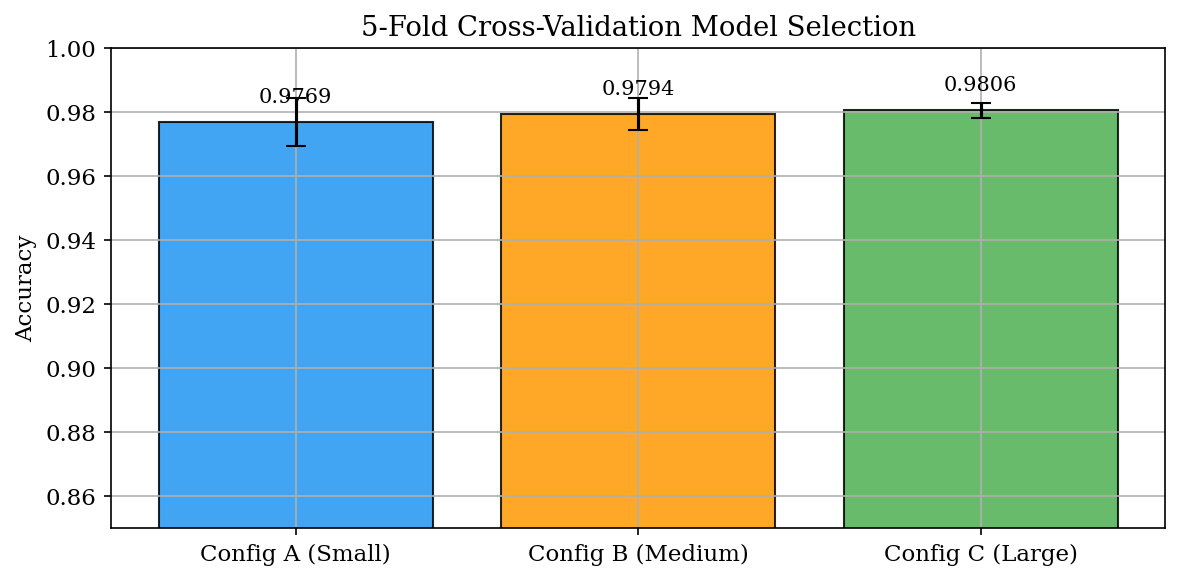
\includegraphics[width=0.65\textwidth]{cv_model_selection.png}
	\caption{5-Fold CV accuracy for the three configurations. Config C achieves the highest mean accuracy with the lowest variance.}
	\label{fig:cv_selection}
\end{figure}

\subsection{Comparison of Selection Approaches}
The TVT approach selected Config B (97.50\% test accuracy) while CV selected Config C (97.75\%), demonstrating that CV provided a more discriminating selection. The TVT approach suffered from a validation set too small to distinguish models whose true errors differ by less than 1\%. CV uses all data for evaluation, providing more reliable estimates aligned with the validation error minimization theory (Lecture 8, slide 11--15).

This result also illustrates the \textbf{complexity--sample size tradeoff} (Lecture 8, slides 7--8). The error of a designed classifier decomposes as $\varepsilon_{n,\mathcal{C}} = \varepsilon^* + \Delta_{\mathcal{C}} + \Delta_{n,\mathcal{C}}$, where $\Delta_{\mathcal{C}}$ is the approximation error (smaller for more complex $\mathcal{C}$) and $\Delta_{n,\mathcal{C}}$ is the design error (larger for more complex $\mathcal{C}$ at fixed $n$). With $n = 1600$ samples, Config C's larger classifier space ($|\mathcal{C}|$, 90K parameters) achieves a lower $\Delta_{\mathcal{C}}$ without incurring excessive $\Delta_{n,\mathcal{C}}$, because the strong dropout (0.4) effectively constrains the functional complexity. For a smaller dataset, the simpler Config A would likely be preferred, as the design error would dominate.

\section{Conclusion}
A fully connected neural network with ReLU activations, batch normalization, and dropout achieves 97.75\% accuracy on the mfeat-factors 10-class digit classification task. The error estimation experiments confirm that resubstitution is severely optimistically biased (0.00\% vs.\ true 1.75\%), hold-out partially corrects this (0.62\%) but remains optimistic due to single-split limitations, and 5-fold CV provides the most reliable estimate (2.50\%) with slight pessimistic bias from the reduced training set size, as predicted by $E[\hat{\varepsilon}_n] = E[\varepsilon_{n-n/k}]$ (Lecture 7). The quantitative RMS bound of $\leq 2.80\%$ for hold-out with $m=320$ samples confirms that error estimation precision is fundamentally limited by validation set size. For model selection, cross-validation proved more discriminating than train-validation-test splitting: the selection probability theorem shows that TVT's 240-sample validation set yields a vacuous bound, while CV effectively uses all 1600 samples. The selected model (Config C) achieves the best tradeoff in the complexity--sample size decomposition $\varepsilon_{n,\mathcal{C}} = \varepsilon^* + \Delta_{\mathcal{C}} + \Delta_{n,\mathcal{C}}$ (Lecture 8), with higher capacity regularized by stronger dropout.

\end{document}
